\section*{Introduction}

%%Motivation: spatio temporal analysis common. Cdc reports. Can these be automated

Large-scale spatio-temporal analysis and forecasts are becoming increasingly common for several diseases,
such as, Influenza \cite{chakraborty:sdm14, wang:kdd16, tizzoni2012real, brooks:ploscb15} and Dengue \cite{johnson2018}.
There is a lot of public interest in analysis of spatio-temporal trends
relating to how these diseases are spreading across the US.
Such analysis includes statements about whether the season has officially 
started, a listing of regions which have differing levels of activity,
the contrast between the current season and earlier seasons, 
and different kinds of trends.
Such analyses have a broad readership,
and are popular among news media, the general public, government agencies,
as well as public health related organizations; 
this is evidenced by the following
examples of spatio-temporal patterns about the spread of Influenza from
news agencies and blogs:
\begin{quote}
For three weeks straight, the health departments of 49 states
--- all except Hawaii --- have reported ``widespread'' flu activity
--- New York Times~\cite{nytimes}
\end{quote}
\begin{quote}
Of the Lower 48 states, Oregon is the only one reporting ``regional''
flu activity for the week ending Jan. 27. For every other state in the contiguous
U.S., flu activity remains ``widespread.'' --- Mashable~\cite{mashable}
\end{quote}

Such patterns are typically identified manually by domain experts,
who have significant expertise on specific diseases.
Data for such analyses often comes from public health agencies,
such as the Centers for Disease Control (CDC) and
World Health Organization (WHO)~\cite{cdc:surveillance-report-feb10}.
Reports generated by CDC contain raw surveillance data on metrics, e.g.,
activity level from outpatient visits and rates of hospitalization,
across states in the US.
In addition, summaries of regions with specific characteristics,
e.g., those which have high activity levels, are also included in the reports.
Following are a couple of such summaries from CDC reports, which are visualized in Figure \ref{fig:summaries}:
\begin{quote}
14 states (Alabama, Arkansas, Georgia, Kansas, Kentucky, Louisiana, Mississippi, North Carolina, Oklahoma, Rhode Island, South Carolina, Tennessee, Texas, and Virginia) have experienced high ILI activity
--- CDC Report for week ending Mar 04, 2017~\cite{cdc:surveillance-report-mar04}.
\end{quote}
\begin{quote}
$\ldots$ and 43 states experienced high activity
(Alabama, Alaska, Arizona, Arkansas, California, Colorado, Connecticut, Delaware, Florida, Georgia, Illinois, Indiana, Iowa, Kansas, Kentucky, Louisiana, Maryland, Massachusetts, Michigan, Minnesota, Mississippi, Missouri, Nebraska, Nevada, New Hampshire, New Jersey, New Mexico, New York, North Carolina, Ohio, Oklahoma, Oregon, Pennsylvania, Rhode Island, South Carolina, South Dakota, Tennessee, Texas, Vermont, Virginia, West Virginia, Wisconsin, and Wyoming)
--- CDC Report for the week ending Feb 10, 2018~\cite{cdc:surveillance-report-feb10}.
\end{quote}

\begin{figure}[!ht]
\centering
\subfloat[Subfigure 1 list of figures text][Mar 04, 2017]{
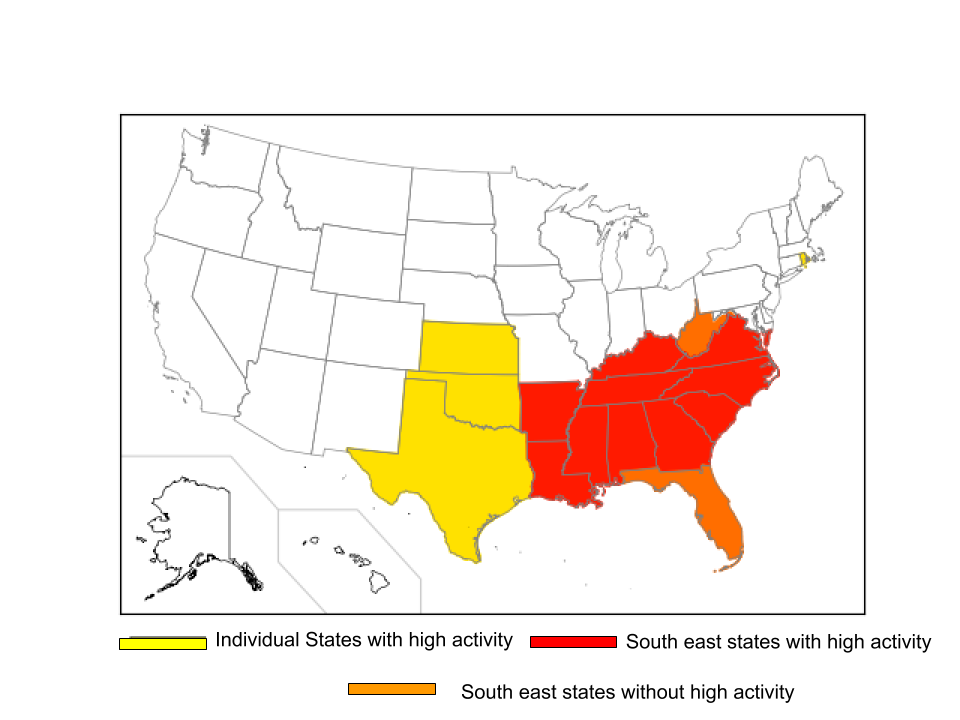
\includegraphics[width=0.5\textwidth]{./figures/mar04.png}
\label{fig:mar04}}
\subfloat[Subfigure 2 list of figures text][Feb 10, 2018]{
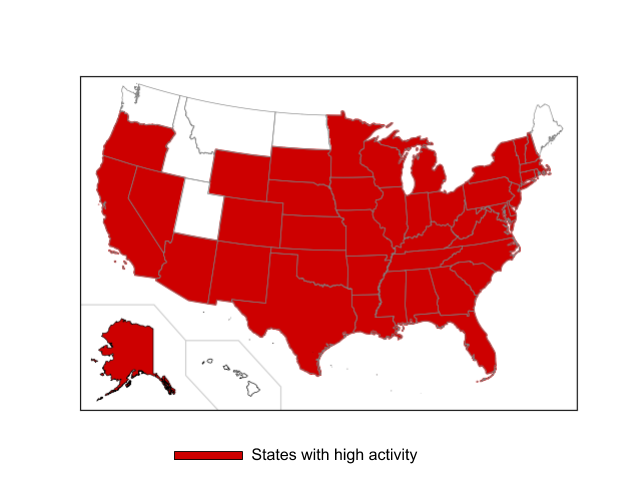
\includegraphics[width=0.5\textwidth]{./figures/feb10.png}
\label{fig:feb10}}
\caption{
Illustration of possible succinct descriptions of the sets of states with
a high ILI activity levels in the weeks of 
(a) Mar 04, 2017: this consists of all the South East states,
except for Florida and West Virginia (shown in red and orange, respectively), 
and the states of Texas, Rhode Island, Kansas, Oklahoma
(shown in yellow);
(b) Feb 10, 2018: this consists of all US states, except 
Washington, Idaho, Utah, Montana, North Dakota, Maine, and Hawaii
(shown in red).
}
\label{fig:summaries}
\end{figure}

The descriptive listings presented above are easy to construct from raw data,
but are tedious to read and do not provide deeper insights into how the
disease is spreading.
In contrast, the analysis by Mashable~\cite{mashable} mentioned
earlier is a \emph{succinct} description
of the set of states which have widespread activity,
namely, all states in the contiguous U.S., except Oregon.
The analysis by the New York Times~\cite{nytimes} mentioned earlier
is also a good and succinct description
of the set of states which have reported widespread activity for three consecutive weeks. 
Figure \ref{fig:summaries} presents succinct descriptions 
of the states with high ILI activity levels for the weeks of 
Mar 04, 2017 and Feb 10, 2018, which contrast with the simple listings by CDC
mentioned earlier.

In addition to descriptions of the set of states with a particular activity
level sets exhibiting specific temporal patterns might also be of interest.
An example is the set of states which maintained a 
stable high activity for three consecutive weeks, ending in the week of 
January 27, 2018:
\begin{quote}
Most states which had high ILI activity level four weeks back,
plus the states of New Jersey, New Mexico, Virginia, Washington, Wyoming.
\end{quote}
This is illustrated in Figure \ref{fig:jan27}. Note that two of the
states which had a high ILI activity level four weeks back, namely,
Nebraska and Tennessee did not exhibit the high level for subsequent
three weeks, which is the reason the description involves ``most'' such states.

%%The description of states that follow a pattern might be of use to the public health and other domain experts. One such pattern could be a set of states that maintain stable high activity for three consecutive weeks. Below is a description of states following this pattern for the week of January 27, 2018, also presented in the Figure \ref{fig:jan27}.
%%\begin{quote}
%%New Jersey, New Mexico, Virginia, Washington, Wyoming and states with high four weeks ago excluding Nebraska and Tennessee 
%%\end{quote}

\begin{figure}[!ht]
\centering
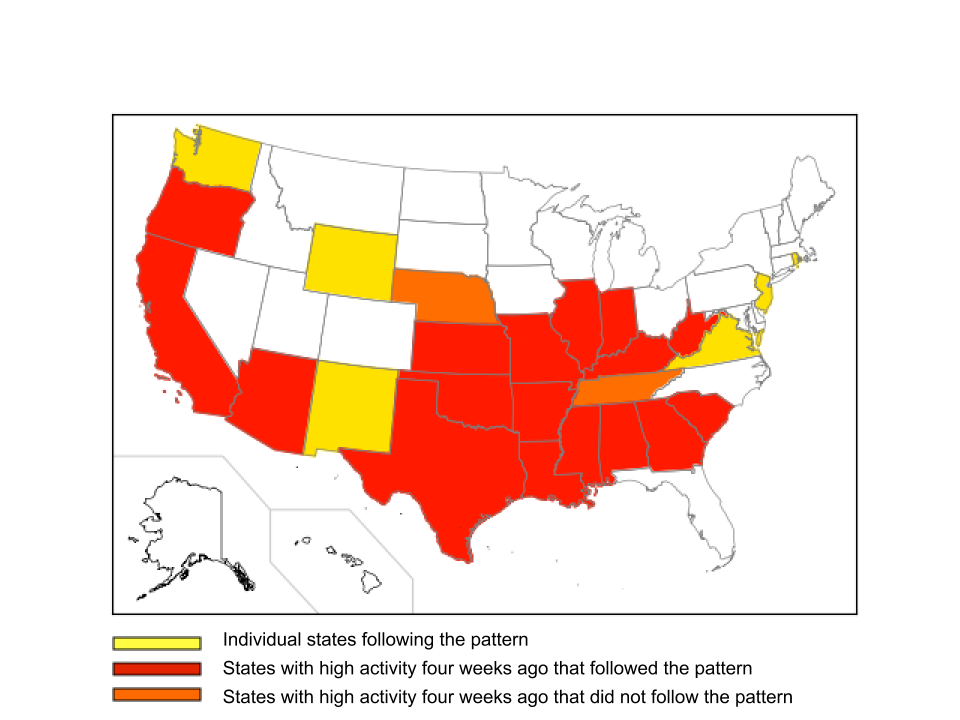
\includegraphics[scale = 0.4]{./figures/jan27.png}
\caption{
The set of states with high ILI activity level for three consecutive
weeks, ending in the week of January 27, 2017: all the states
which were at high four weeks back, except Nebraska and Tennessee
(shown in red and orange, respectively), and the five states are shown in yellow.
}
\label{fig:jan27}
\end{figure}

The overall objective of our work is to automate the process of
identifying ``interesting'' spatio-temporal patterns from 
disease surveillance data,
and generating succinct descriptions for them.
We use the approach of mining patterns from transactional data
for formalizing these questions, which has been successfully used 
in many areas, such as analysis of retail transaction data \cite{assocmining},
biomedical data analysis \cite{madeira1, xiang:dmkd2011}, and information retrieval \cite{infretr2004}.

These data sets can be encoded as a binary $n\times m$ matrix $D$,
where the $n$ rows represent transactions and the $m$ columns 
represent items. The $i$th transaction corresponds to the $i$th row of $D$, and
consists of a subset of items (which have value $1$ in the corresponding
entry).
A general approach of summarizing the entries of the transaction-item matrix $D$ is via clustering.
Such clusters can then be used for pattern analysis. In \cite{chandola:icdm05}, authors formulate the problem of summarizing a transactional dataset as an optimization and approach it via clustering and association analysis. Some later works use MDL principle such as \cite{Vreeken2011, miettinen2011} to find the set of patterns that compress the dataset best.

The main contribution of this paper is
a novel approach for finding patterns in epidemic incidence data.
Using the techniques of pattern mining in transactional data, we interpret the incidence data
as a transaction-item matrix and develop an integer programming based technique for finding 
``succinct'' descriptions for a given subset of regions.
An automated method is desgined for searching 
different sets of regions, and identifying patterns of interest
by considering those which have the most succinct descriptions.
The Influenza incidence data for the US, obtained from Centers for 
Disease Control (CDC)~\cite{cdc:surveillance-report-feb10} is used to illustrate
our methods. A brief description of this data is presented in both the methods and the
results sections.


